\articlehead{A Bitch About Furry}{JM}{2013}

Tolerance is one of the great features of the furry community.

We need to be tolerant. Our community contains a lot of people who are sometimes marginalized in general society: gays, transsexuals, zoophiles, kinksters, even geeks.

This tolerance is sometimes positive acceptance, but it's often simply neutral, the absence of rejection. Furry behaviour is often more tolerant than general society simply through such tacit acceptance. This is clearly demonstrated by the language we use, especially online where less direct methods of communication are less significant. Put simply, intolerant or offensive language is not appropriate in furry spaces.

There is one significant exception: women. Some furries, especially online, use sexist language. Worse, it's being ignored, perhaps tacitly accepted, which fosters an environment which is unwelcoming towards women. Furry culture might reasonably be considered a sexist one.

To clarify: I do not think that furries are sexist. But I do think sexist language is common within furry.

To start with, I'd like to compare sexist language with other offensive terms:

\begin{enumerate}
  \item Faggot

  \begin{itemize}
    \item It is a homophobic term, largely because of the inherent implication that being gay makes you less of a person.
    \item It has aggressive, confrontational connotations that suggests gay men are not welcome.
    \item Once commonly used, it has fallen from favour through the indirect forces of political correctness.
    \item Anyone using the word `faggot' in a furry space can expect to be shouted down.
  \end{itemize}

  \item Nigger

  \begin{itemize}
    \item It is a racist term, largely because of the inherent implication that being black makes you less of a person.
    \item It has aggressive, confrontational connotations that suggests black people are not welcome.
    \item Once commonly used, it has fallen from favour through the indirect forces of political correctness.
    \item Anyone using the word `nigger' in a furry space can expect to be shouted down.
  \end{itemize}

  \item Bitch

  \begin{itemize}
    \item It is a sexist term, largely because of the inherent implication that being female makes you less of a person.
    \item It has aggressive, confrontational connotations that suggests women are not welcome.
    \item Once commonly used, it has fallen from favour through the indirect forces of political correctness.
    \item Yet `bitch' is fairly common in furry circles.
  \end{itemize}
\end{enumerate}

A quick semantic aside: `bitch' can refer to a female dog. This makes it an appropriate term under some circumstances, much in the same way that a sheep might be referred to as a ewe. This usage is not relevant to the use of bitch as a sexist term.

(I'll add that `faggot' is a fairly common British word: it's a kind of meatball made from liver, lungs, heart, and stomach lining. Yum.)

I have a couple of examples of furries using `bitch' in public forums. Both are recent.

The first is from a Flayrah comment thread, written in response to an article on a recent death in the fandom. Please note that the comment is a blunt and emotional one (not that Flayrah comment threads are typically known for their dispassionate nuance), however that's not my focus.

41-bitch1

Tim's comments are directed towards the driver of a car involved in a fatal accident. She survived. The comment is angry, then becomes offensive with the sexist language exacta: `bitch' and `cunt'. There two words suggest that Tim believes the driver's gender is relevant, and perhaps partially to blame.

Tim's terminology suggests that he is angered by the driver's gender as much as by the accident itself. Many women reading his comment will have felt that anger directed towards them, by association.

Nobody comments on Tim's sexist language, although he does get reprimanded for being generally unreasonable: someone steps into to call him a `stupid asshole', at which point a moderate intervenes.

\begin{figure}
  \begin{center}
    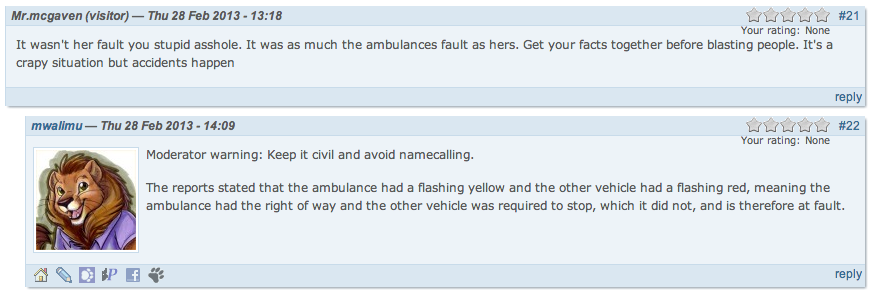
\includegraphics[width=\textwidth]{content/assets/bitch--comments}
  \end{center}
  \caption{Flayrah comments}
\end{figure}

(I've edited some intervening comments in the thread for clarity: you can see the full exchange here.)

To keep this in context, this is a nothing but a comment thread on an emotive topic, no more than poorly-thought-out expressions of anger and impotent frustration. However I think it's instructive that Tim's sexist language was ignored while the namecalling wasn't. Consider if Tim had used homophobic language, something the furry community doesn't tolerate: if the driver of the car were gay, and Tim had called him a `faggot', his language would have been firmly corrected (and Flayrah's comment-rating system's six votes wouldn't have scored him 3/5).

My second example is a tweet sent out by a friend of mine:

\begin{quotation}
  I'm met this bitch before, she snatches shit out of other customers hands and then snarls at them like a rabid dog. Fucking crazed OAP bitch\\
  -- Sphelx Komodo (@sphelx) March 2, 2013
\end{quotation}

I asked Sphelx about his comment, and he told me that the sexist slur was at least partly deliberate (``I don't really see how [bitch] is explicitly sexist, at least anymore\ldots I think it's been replaced with `cunt'\ldots I was actually going to say `cunt' at first, but then I decided to tone it down''), but that his general intent was to express anger, not to be offensive.

Sphelx is not a fundamentally sexist person. He has used this sexist language for the same reason that many furries use it: he has not been exposed to a coherent argument explaining why it's harmful.

He's hardly Robinson Crusoe. His language is pretty typical of a visible minority in the furry community. Behaviour only changes if it is challenged, and challenged in a friendly and non-judgmental fashion, which allows the person to consider the counterargument in their own way and in their own time.

It's easy to take sides and look at such people as `wrong', or `bad', especially when you don't know them. But it's worth considering that the world doesn't contain many people who identify as sexist. (A common refrain is some variation of “I'm not sexist, I love women”, a phrase comparable to “I'm not homophobic, some of my best friends are gay”.) And if someone doesn't think of themselves as sexist, a direct accusation will simply provoke a defensive reaction, likely followed by a frustrating and counterproductive argument.

The issue here is not enforcement of universal goodthink, it's simply language and behaviour. A good person like Sphelx looks intolerant when he uses sexist language. If you wish to challenge someone, challenge the issue—their language and behaviour—not their thoughts or motivations.

Furries, being rather young and male and techy, get exposed to a lot of fundamentally sexist online cultures. The gaming subculture is one overt example, but there are many others. Such online communities are often informed by the so-called `men's rights' movement.

The men's rights movement is a crude backlash against feminism. It challenges discrimination applied against men, presuming that the forces challenging discrimination against women are sufficient. Such groups are essentially the gender-based equivalent of other contrarian equality movements, using the logic that steps taken to help female/black/gay people are discriminatory in themselves, and that we should all be gender/race/sexuality blind. They are typically focussed on positive discrimination measures, or government spending on minorities: examples include women-only gyms, racial quotas, and LGBT-only support.

Concerns over such discrimination would be spot on, except for the fact that this isn't Star Trek. Discrimination towards women (and gay people, and racial minorities) exists, and action needs to be taken to reverse this discrimination.

Men's rights groups frame the problem in an us-versus-them fashion: they see feminism as an extremist movement driven to help women at the expense of men. Similarly, nationalist political groups think that there is an extreme movement to help racial minorities at the expense of the majority. And (some) religious groups think that there is an extreme movement to help homosexuals at the expense of heterosexuals. I'd argue that they are misguided but, fundamentally, they are all driven by the desire for fairness: in this way, the goal of men's rights groups and feminists is the same.

Consider a hypothetical gender quota, where an employer must hire a certain percentage of women in an otherwise male-dominated field (perhaps IT, or politics, or business). In such a field, senior management tends to be almost exclusively male, simply because of mathematics: there are far more men with experience to choose from. A general lack of women means that any new female starter will be an immediate outsider; a dearth of women in upper management means that she has limited role models.

(In comparison, it is a lot easier to be a black highschool quarterback nowadays, compared to the 1980s. An aspiring black quarterback is no longer so unusual: a black quarterback is now simply a quarterback.)

Recognizing that it is more difficult for women entering a male-dominated field (because of their outsider status and lack of role models), recruiters can choose to hire a greater proportion of women. This has two positive effects: firstly, they will be hiring women who have reached that point in spite of their inherent disadvantages; secondly, they will be creating a workplace with more female role models, reducing and ultimately removing the problem.

This is all great, except when you're the talented male candidate who is passed over for a less capable woman. And it's easy to see the trees, ignore the wood, and conclude that the system is sexist against men. It's not.

Certainly such a system is discriminatory, and the man is being discriminated against. However this is in recognition of the discrimination against women that takes place in a less direct fashion. In an ideal world -- Star Trek again -- neither form of discrimination would occur, and gender politics wouldn't play any part. We don't live in such a world, but we're getting there, and positive discrimination accelerates its arrival.

Feminism isn't about the rise of women over men: it's intelligent humanism. The ways in which the world discriminates against women are subtle, complex, and ever-changing. Feminism is a reaction to that.

The furry community doesn't have much of a visible feminist element, but we should. A friendly flock of furry feminists would help us improve our collective behaviour towards our female minority. Language is one of the easiest ways that we can improve. Let's start by consigning `bitch' to the same scrapheap as `faggot'.
